\documentclass[12pt]{article}

\title{ECE4063 - Image Thresholding}
%\subtitle{Progress Report}
\author{Emmanuel Jacyna - 24227498 \and James Anastasiou - 23438940}
\date{\today}

\usepackage[T1]{fontenc}
\usepackage[utf8]{inputenc}
\usepackage{rotating}
\usepackage{subfig}

\usepackage{graphicx}
\usepackage{tabularx}
\usepackage{float}
\usepackage{amsmath}
\usepackage{listings}
\bibliographystyle{unsrt}


\begin{document}
\pagestyle{myheadings}
  \maketitle
  \tableofcontents
  \section{Introduction}
  This document represents our findings for Assignment 2 of ECE4063. It is organised into three major sections, assumptions, solution documentation, and a discussion of potential improvements to the project.\\
  
  The task at hand is to perform binary thresholding on an image for use in a bionic eye. The target platform is an Altera Cyclone II FPGA. In order to threshold the image, a histogram of the pixel greyscale values is calculated and used to find the 50th percentile grey scale value. This value is then used to decide whether to colour pixels white or black, performing a total threshold.
  
  \section{Assumptions}
  When thresholding images, we assume that an image where 99.9\% of pixels are one value is meaningless to threshold. In the case of the Altera DE2 board with Terasic camera module, the small variation in value is likely to be because of pixel noise. We also believe that as the target is a human vision system, 100\% accuracy is not necessarily the goal, as we prefer an image that makes sense to the human eye. This design decision allowed for a simplification of the logic circuit required to determine the most accurate thresholding value. 
  
  We also assumed that Model Sim testbenches are 100\% completely accurate representations of reality. This assumption was routinely called into question, however after fixing a number of other assumptions, this sole assumption was found to be a valid assumption.
  
  \section{Documentation}
  \subsection{RGB to Grayscale conversion}
  
  \subsection{Histogram Module}
  The histogram module was 
  
  \subsubsection{Module Testbench Results}
  
  \subsection{Cumulative Histogram Module}
  
  \subsection{Thresholding Module}
  \subsubsection{Description}
  The thresholding module is very simple. All it needs to do is take in an 8 bit greyscale value and output either a white (255) if the value is above the threshold, or a black (0) if the value is below the threshold. This is accomplished by hooking up a comparator to a multiplexer.
  
  \subsubsection{RTL Diagram}
  \begin{figure}[H]
    \centering{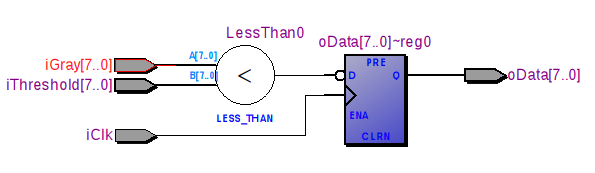
\includegraphics[scale=.8]{Images/ThresholderRTL.png}}
    \caption{Thresholding module RTL}
    \label{fig:thresholder_rtl}
  \end{figure}
  
  
  \subsection{Displaying things}
  \subsubsection{Description}
  In order to display the greyscale image, histogram, cumulative histogram, and thresholded image, we wrote a module to handle multiplexing between them using the switches on the DE2 board, called Arbitrator. This module takes in pixel outputs from the various modules and multiplexes them depending on the switch positions. In order to display images, we simply piggyback on the \(X\_Cont\) and \(Y\_Cont\) signals and modify the \(wr1\_data\) and \(wr2\_data\) inputs to the SDRAM with the appropriate pixel data. \\
      
  Displaying the actual histogram data requires slightly more effort. First we need to extract the histogram data from the histogram RAM and convert the histogram bin contents into pixels for display on the screen. To do this we have a module called HistogramDisplayer. This module takes in the \(Y\_Cont\) signal and uses it to index the histogram RAM. Based on the value obtained from the RAM, it scales the histogram value, and uses the \(X\_Cont\) signal to determine the length of the line to be displayed. 
  \subsubsection{RTL Diagram}
    \begin{figure}[H]
    \centering{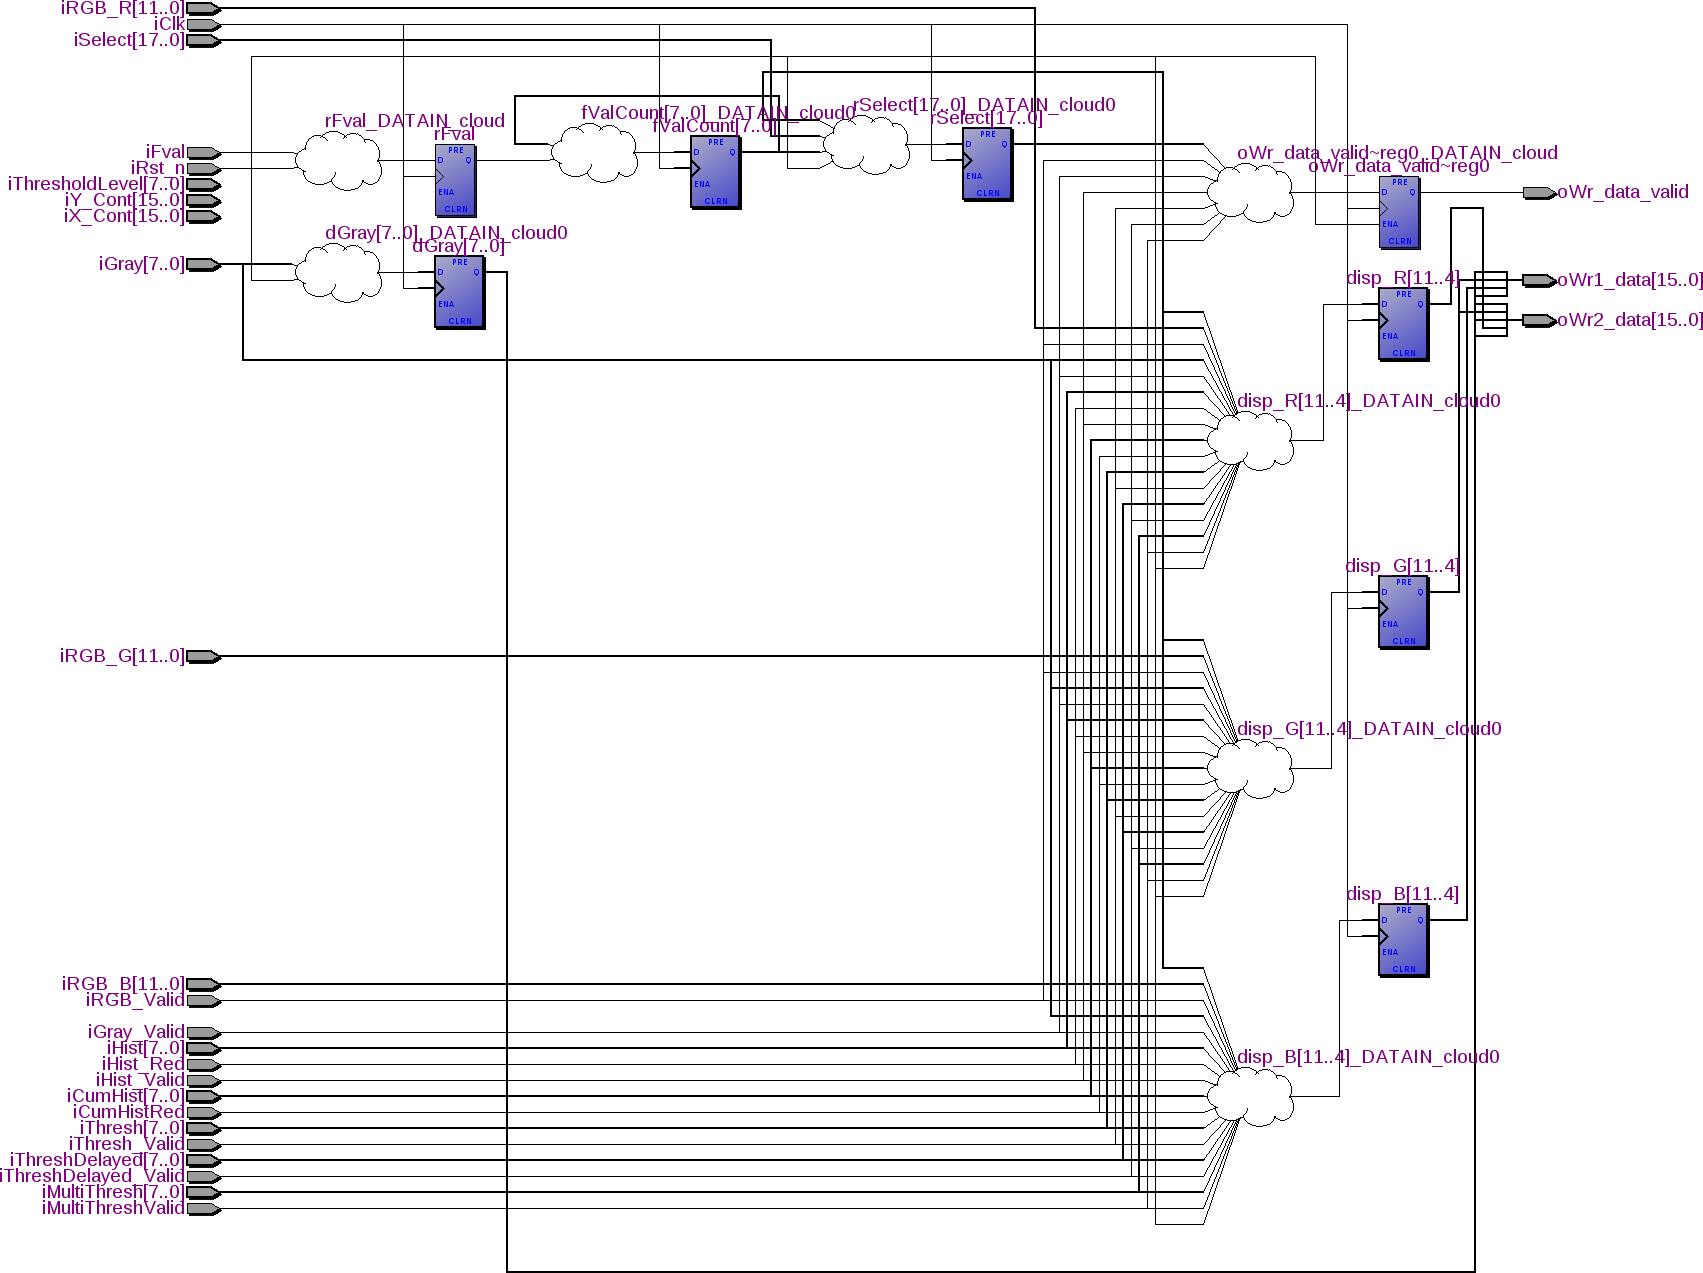
\includegraphics[scale=.8]{Images/ArbitratorRTL.png}}
    \caption{Arbitrator module RTL}
    \label{fig:arbitrator_rtl}
  \end{figure} 
  \subsubsection{RTL Diagram}
    \begin{figure}[H]
    \centering{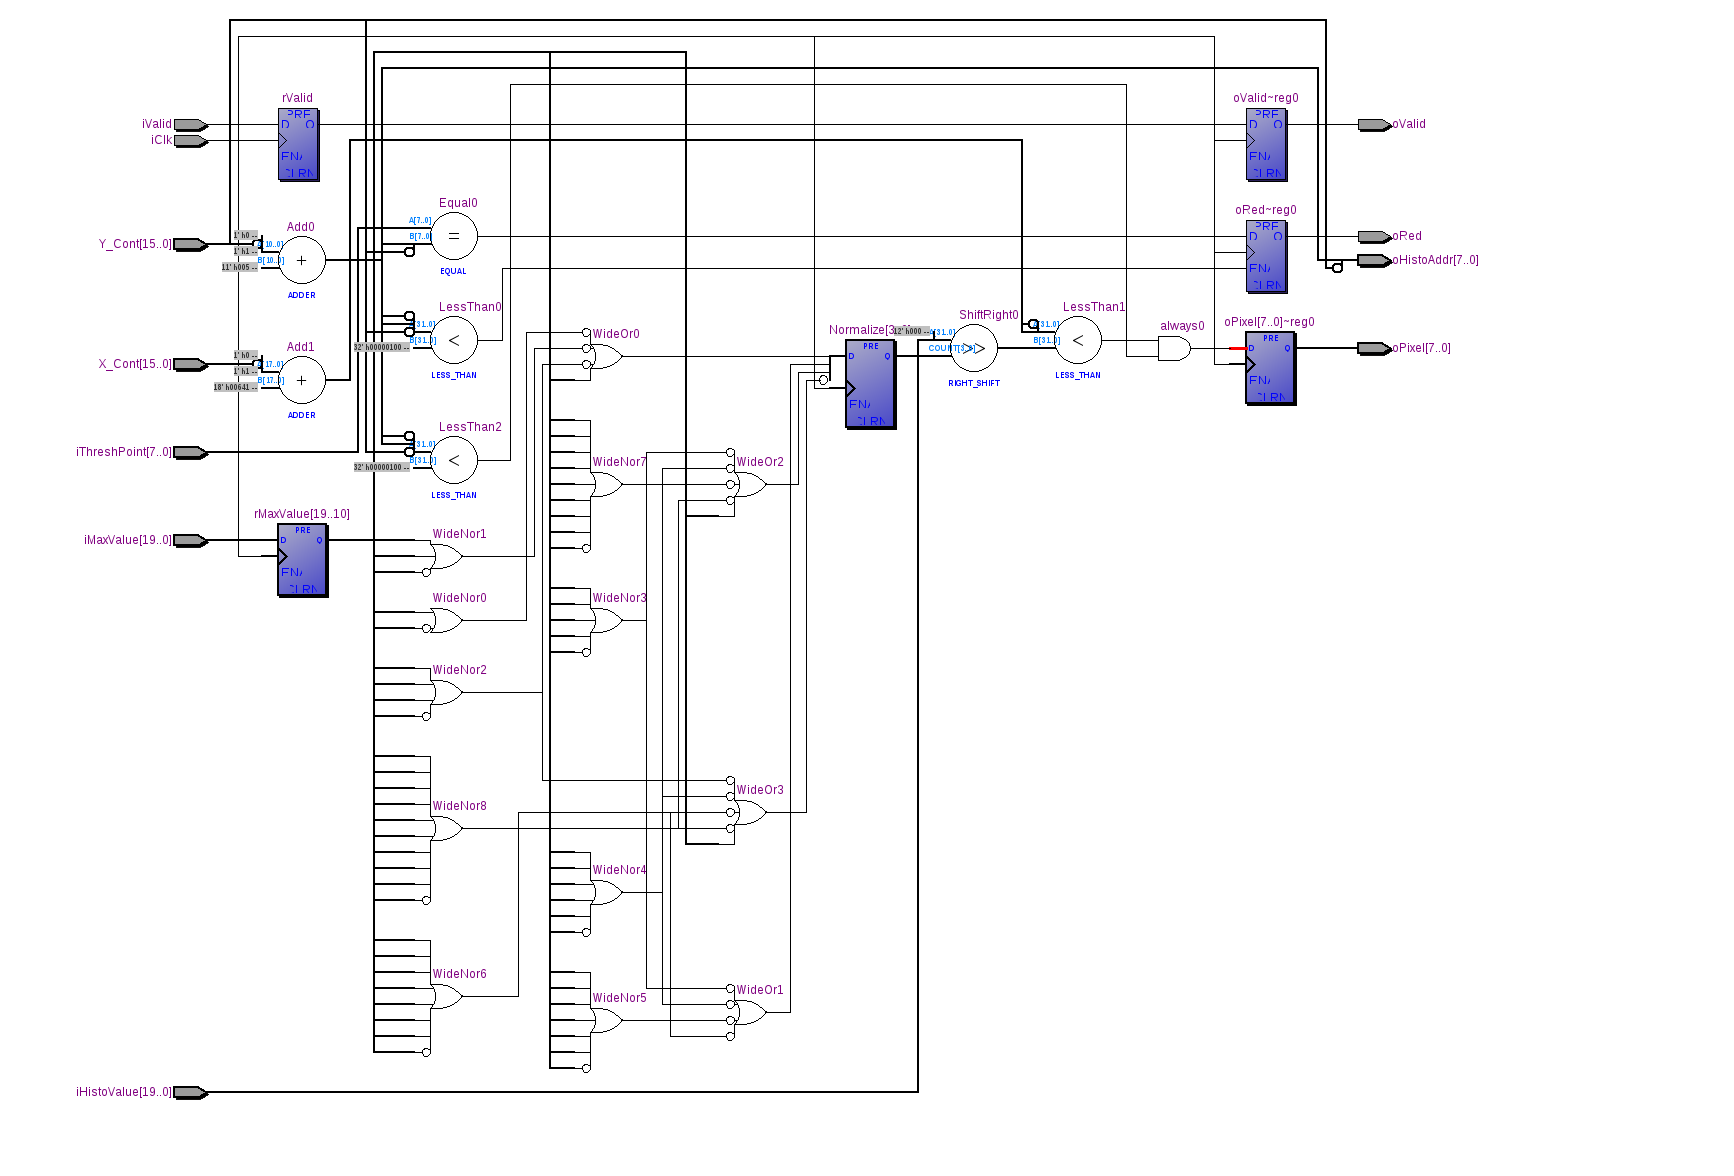
\includegraphics[scale=.8]{Images/HistogramDisplayerRTL.png}}
    \caption{HistogramDisplayer module RTL}
    \label{fig:histogram_displayer_rtl}
  \end{figure}
  
  \section{Acknowledgements}
  
  \section{Improvements}
  
  \section{Conclusion}
  
  \newpage
  \section{Appendix A}
  \subsection{RTL Diagrams}
  \subsubsection{Histogram}
  \begin{figure}[H]
    \ContinuedFloat
    \centering{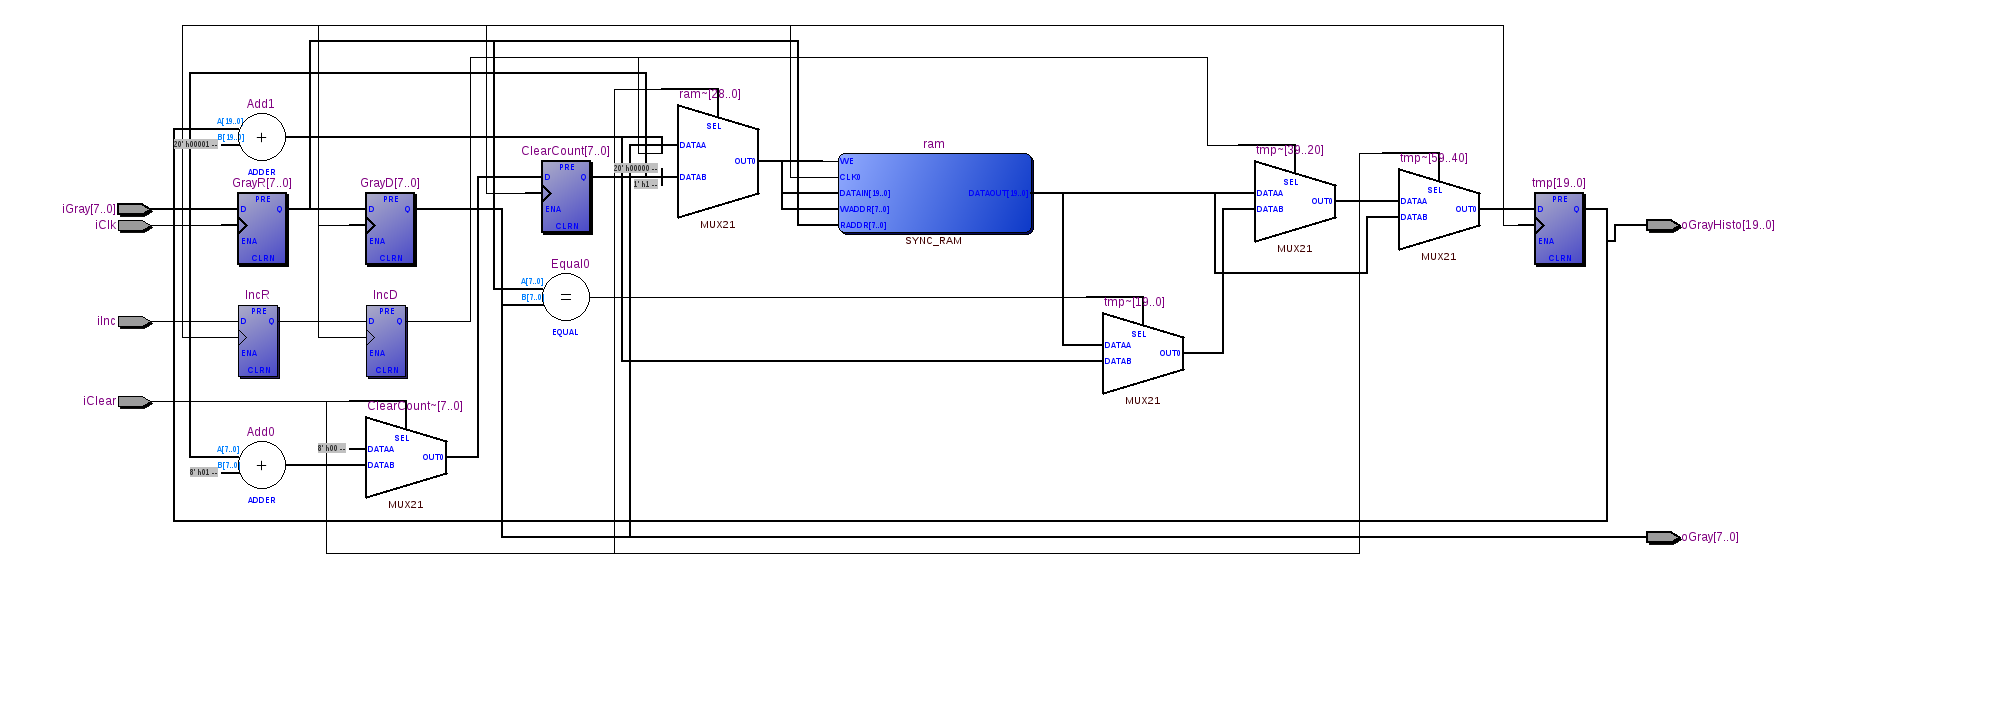
\includegraphics[scale=.6, angle=-90]{Images/HistogramRTL.png}}
    \caption{Histogram module RTL}
    \label{fig:histogram_rtl}
  \end{figure}
  
  
  
  
\end{document}
